\documentclass[fleqn,12pt]{article}
\usepackage[top=2cm, left=2cm,right=2cm,bottom=2cm]{geometry}
%\usepackage[fleqn]{amsmath}
\usepackage{amsmath}
\usepackage{url,multicol}
\usepackage{enumerate}
\usepackage{ifthen}
\newboolean{answers}
%\setboolean{answers}{true}  % set to true to include TODO statements
\setboolean{answers}{false}  % set to false to use input statements
\usepackage{amssymb}
\usepackage{tikz}
\newcommand{\<}{\ensuremath{\langle}}
\renewcommand{\>}{\ensuremath{\rangle}}
\newcommand{\ur}{\ensuremath{\underline{\mathrm{r}}}}
\newcommand{\uT}{\ensuremath{\underline{\mathrm{T}}}}
\newcommand{\uF}{\ensuremath{\underline{\mathrm{F}}}}
\newcommand{\uN}{\ensuremath{\underline{\mathrm{N}}}}
\newcommand{\ui}{\ensuremath{\underline{\mathrm{i}}}}
\newcommand{\uj}{\ensuremath{\underline{\mathrm{j}}}}
\newcommand{\ua}{\ensuremath{\underline{\mathrm{a}}}}
\newcommand{\ub}{\ensuremath{\underline{\mathrm{b}}}}
\newcommand{\un}{\ensuremath{\underline{\mathrm{n}}}}
\newcommand{\uv}{\ensuremath{\underline{\mathrm{v}}}}
\newcommand{\ba}{\ensuremath{\mathbf{a}}}
\newcommand{\bv}{\ensuremath{\mathbf{v}}}
\newcommand{\bb}{\ensuremath{\mathbf{b}}}
\newcommand{\bc}{\ensuremath{\mathbf{c}}}
\newcommand{\bi}{\ensuremath{\mathbf{i}}}
\newcommand{\bj}{\ensuremath{\mathbf{j}}}
\newcommand{\dotsize}{1pt}
\usepackage{fancyheadings}
\begin{document}
%\thispagestyle{empty}
%\pagestyle{empty}
\pagestyle{fancyplain}
%% \lfoot[\fancyplain{{\small score: \underline{\phantom{XXXX}}}}{{\small score: \underline{\phantom{XXXX}}}}]                 {\fancyplain{}{}}
\lhead[]{}\chead[]{}\rhead[]{}
\lfoot[{\small score: \underline{\phantom{XXXXXX}}}]{{\small score: \underline{\phantom{XXXXXX}}}}
\cfoot[]{}
\rhead[]{For full credit, SHOW YOUR WORK.}
\lhead[Math 160: Fall 2015]{Math 160: Fall 2015}

%\fontsize{11.5}{13.8}
% \fontsize{14}{17}
% \selectfont
\noindent {\bf MATH 160}
\hfill {\bf Fall 2015}
\begin{center}
{\bf EXAMINATION 3}
\thispagestyle{empty}
%% covers sections 5.1--5.5 and 7.1--7.4
\end{center}
\vskip1cm
\noindent {\bf RULES}
\begin{itemize}
\item No books or notes or calculators allowed.
\item No bathroom breaks until after you have completed and turned in your exam.
\item Out of consideration for your classmates, do not make
disturbing noises during the exam.
\item {\bf Phones must be turned off.}
\end{itemize}
\vskip1cm
{\it Cheating will not be tolerated.}  If there are any indications that a
  student gave or received unauthorized aid on this test, the case 
  will be referred to the ISU Office of Judicial Affairs.% \\
\\\\
When you finish the exam, please sign the following statement acknowledging that
you understand  this policy:\\
\\
``On my honor as a student I,
\underline{\phantom{XXXXXXXXXXXXXXXXXXXX}}, have neither
given nor received aid on this exam.''
\hbox{} \hskip 1in {\small (carefully print full name)}\\
\\
\begin{flushright} Signature: \underline{\phantom{XXXXXXXXXXXXXXXXXXXXXXXX}}
  Date: \underline{\phantom{XXX}2015/12/01\phantom{XXX}}
\end{flushright}

\vskip3cm
%% \begin{flushright}
\begin{center}
  {\Large
\begin{tabular}{r|c|c|l}
page   & problems & max  & score\\[4pt]
\hline
1 & 1--2 &20&\\[4pt]
\hline
2 & 3--5 &20&\\[4pt]
\hline
3 & 6 & 12&\\[4pt]
\hline
4 & 7 & 10&\\[4pt]
\hline
5 & 8 & 8&\\[4pt]
\hline
total & & 70&
\end{tabular}
}
%% \end{flushright}
\end{center}


\newpage
\begin{enumerate}
\item %%% Problem 1. %%%
(8pts)
Find the horizontal and vertical asymptotes of the graph of the function. 
If an answer does not exist, write DNE.  
(You must show your work and justify your answer,
but you need not sketch the graph.) 
\[
g(x) = \frac{x^3}{x^2-3}
\]
\vskip3cm
\ifthenelse{\boolean{answers}}{
\hfill horizontal asymptote(s): \underline{\phantom{XX}DNE\phantom{XX}}\\\\
\strut\hfill vertical asymptote(s): \underline{$x =  ­3$ and $x=3$}
}{
\hfill horizontal asymptote(s):     \underline{\phantom{XXXXXXxXXXX}}\\[20pt]
\strut\hfill vertical asymptote(s): \underline{\phantom{XXXXXXXXXX}}
}

\newcommand\probskip{\vskip1cm}

\probskip

\item %%% Problem 2. %%%
(12pts)
Find the absolute maximum value and the absolute minimum value, if any, of the
function. (If an answer does not exist, enter DNE.)
\[
f(x) = 10x - \frac{3}{x} \quad \text{ on $[1,3]$}
\]
\vfill
\ifthenelse{\boolean{answers}}{
\hfill maximum value: $f(x_{\max}) = \underline{\phantom{XX}29\phantom{XX}}$\\\\
\strut\hfill minimum value: $f(x_{\min}) = \underline{\phantom{XX}7\phantom{XX}}$
}{
\hfill maximum value: $f(x_{\max}) = \underline{\phantom{XXXXXX}}$\\\\
\strut\hfill minimum value: $f(x_{\min}) = \underline{\phantom{XXXXXX}}$
}

  %% \vfill
  %% score: \underline{\phantom{XXXX}/20}

\newpage

\item %%% Problem 3. %%%
(5pts) 
Determine whether the statement is true or false and check the
  box next to the correct statement explaining why it's true or false.  (You
  need not show your work for this problem.)

  \begin{quote}
  If $f''(x) < 0$ on $(a, b)$ and $f'(c) = 0$ where $a < c < b$, then $f(c)$ 
  is the absolute \emph{maximum} value of $f$ on $[a, b]$.
  \end{quote}

\noindent $\square$ True. 
$f''(x) < 0$  on $(a, b)$ says that the graph of $f$ is concave downward on 
$(a,b)$.  $f'(c) = 0$ means that the graph is not continuous at $c$, that it goes toward infinity. 
Therefore, $f(c) =  \infty$  is the absolute maximum value.\\[5pt]
$\square$ True. 
$f''(x) < 0$  says that the graph is concave downward on $(a, b)$. 
Therefore, the relative maximum value at  $x = c$  must, in fact, be the absolute maximum value.    \\[5pt]
\noindent $\square$ False. If  $b$  is an inflection point where 
$f''(x) = 0$, then the function satisfies the given conditions but has
 absolute maximum value at $b$, not $c$.\\[5pt]
\noindent $\square$ False. Under the given conditions, 
$f(c)$ is the absolute \emph{minimum} value of $f$ on $[a,b]$.\\[5pt]
\noindent $\square$ False.  $f'(c) = 0$  means that the graph is not continuous at $c$,
and that the function tends to infinity. Therefore, it has no absolute maximum value at $c$.

\vskip5mm

\item %%% Problem 4. %%%
(7pts)
Use logarithms to solve the equation for $t$.
\[
6e^{t-5} = 6
\]
\vskip3cm
\ifthenelse{\boolean{answers}}{
\hfill  {\bf Answer:}\hskip.5cm $t = 5$}{
\hfill {\bf Answer:}\hskip.5cm $t = $ \underline{\phantom{XXXXXXX}}}

\probskip
\item %%% Problem 5. %%%
(8pts)
Find the derivative of the function
\[
f(x) = 6x^2 \ln(9x).
\]
\vfill
\ifthenelse{\boolean{answers}}{
\hfill  {\bf Answer:}\hskip.5cm $f'(x) = 6x(1 + 2\ln(9x))$}{
\hfill {\bf Answer:}\hskip.5cm $f'(x) = $ \underline{\phantom{XXXXXXXXXXX}}}

  %% \vfill
  %% score: \underline{\phantom{XXXX}/20}

\newpage
%You must {\bf show your work} for full credit.
\item 
%% Problem 6 %%
(12pts)
Postal regulations specify that a parcel sent by Priority Mail may have a
combined length and girth of no more than 228 inches. 
For a rectangular box with square cross section that may be sent by Priority
Mail, what are the dimensions that give the {\bf maximum volume}?
[{\it Hints:} Recall the formula for volume: (area of
  base)$\times$height or  (area of side)$\times$length. Let $\ell$ denote length and
  let $w$ denote width; then the girth is $4w$.]

    \begin{figure}[!h]
      \begin{center}
      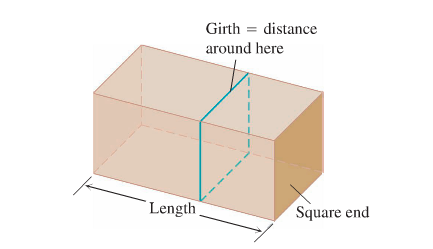
\includegraphics[height=2in]{Prob10-postoffice}
      \caption{Let length + girth $= \ell + 4w = 228$}
      \label{fig1}
  \end{center}
    \end{figure}
\vfill
\hfill {\bf Answer:}\hskip1cm length: $\ell =$ \underline{\phantom{XXXXXXXX}}
\hfill width: $w =$
\underline{\phantom{XXXXXXXXX}}
  %% \vfill
  %% score: \underline{\phantom{XXXX}/20}

\newpage
%For ALL problems on this page, you must {\bf show your work} for full credit.

\item
%% Problem 7 %%
(10pts)
Find the intervals where  $f(x) = x^2e^{-x}$ is increasing and where it is
decreasing. Show your work.  Mark your answers by checking the appropriate boxes below. Select all
that apply. 

\vfill

\begin{multicols}{2}
$f(x)$ is {\bf increasing} on:\\[5pt]
$\square \; (-\infty, 0)  \cup  (2,  \infty )$
%% \\[5pt]
%% $\square \; (-\infty ,  \infty )$    
\\[5pt]
$\square \; (0,  \infty )$
\\[5pt]
$\square\; (-\infty , 0)$ 
\\[5pt]
$\square\; (0, 2)$

$f(x)$ is {\bf decreasing} on:\\[5pt]
$\square\; (0,  \infty )$
%% \\[5pt]$\square\; (-\infty ,  \infty )    $
\\[5pt]
$\square\;  (-\infty , 0)  \cup  (2,  \infty )$
\\[5pt]
$\square\; (0, 2)$
\\[5pt]
$\square\; (-\infty , 0)$
\end{multicols}

\newpage
Solve ONE of either {\bf a.}~OR {\bf b.} then
CIRCLE the letter of the part you want graded.\\[5pt]  If nothing circled, {\bf a.} will be graded.

\item (8pts) 
%% Problem 8 %%
  \begin{enumerate}[{\bf a.}]
  \item Compute the following integrals. (Be sure to give \emph{all} correct antiderivatives by
    including an arbitrary constant $C$ in your answers.)

    \[
    \int 3 \, dx = 
    \]

    \[
    \int x \, dx = 
    \]

  \vskip1cm


  \item
    Sr-90, a radioactive isotope of strontium, is present in the
    fallout resulting from nuclear explosions. It is especially hazardous to animal
    life because, upon ingestion of contaminated food, it is
    absorbed into the bone structure. Its half-life is 24 years. If the amount of 
    Sr-90 in a certain area is found to be four times the safe level, 
    find how much time must elapse before the safe level is reached. 
  \end{enumerate}

\vfill

\ifthenelse{\boolean{answers}}{
\hfill  {\bf Answer:}\hskip1cm \underline{\phantom{XX}48\phantom{XX}} years}{
\hfill {\bf Answer:}\hskip1cm \underline{\phantom{XXXXXXX}} years}

\end{enumerate}

\end{document}
\probskip

\item Find the indefinite integral. (Fill in the blank.)
\[ 
\int 6 dx  = \underline{\phantom{XXXX}} + C.
\]

\begin{center}
  - scratch -
\end{center}

  %% \vfill
  %% score: \underline{\phantom{XXXX}/20}

\newpage
\smallskip
(For example, select (a) $+, 0, -$ if you believe $f''(a)>0$, $f''(b)=0$, and $f''(c)<0$.)
\begin{center}
  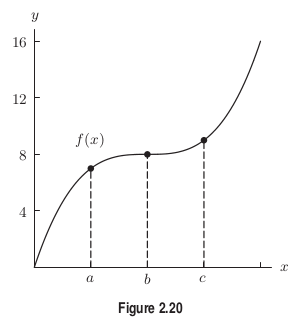
\includegraphics[height=3.5in]{Problem-CT-2-4-9}
\end{center}


\newpage
\end{enumerate}

